\section{Tangles}

\subsection{Tangle diagrams}

Intuitively a tangle diagram is just that: a diagram. One finds a clear area on their paper, draws some lines with some over and under strands in mind. Typically an under strand is denoted by a break in the strand where the crossing should be, we see an example of a tangle diagram in \Cref{fig:tangle_diagram}.

\begin{definition}\textbf{(Tangle diagrams)}
Consider some closed, bounded, convex subset $B\subset\mathbb R^2$, and $n\in\mathbb N$ pairs of points $(a_n,b_n)$ on the boundary of $B$ with $a_i\neq a_j$ and $a_i\neq b_j$ for all $1\le i,j\le n$. Define for each $1\le i\le n$ a map $\phi_i:[0,1]\to B$ such that:
\begin{enumerate}
\item $\phi_i(0)=a_i$, $\phi_i(1)=b_i$, an orientation on the diagram is induced by the orientations of the $\phi_i$,
\item $\phi_i((0,1))\subset B$, i.e the image of $(0,1)$ is fully contained in $B$, we call $\phi_i((0,1))\subset B$ a \textit{strand},
\item We call $c\in B$ a \textit{crossing} if $c$ is in the image of 2 maps $\phi_i$,$\phi_j$, where if $i\neq j$ their preimages $\phi_i^{-1}(c),\phi_j^{-1}(c)$ have only one point, and if $i=j$, then the preimage of $c$ has 2 points. If a point is not a crossing, then it is in the image of at most one map, and its preimage contains a single point,
\item for each crossing $c$ take a neighborhood that contains no other crossing, in the neighborhood designate one \textit{over}, and one \textit{under} strand.
\end{enumerate}
We call this construction an \textit{n-Tangle Diagram}
\end{definition}

\begin{figure}[h!]
\centering
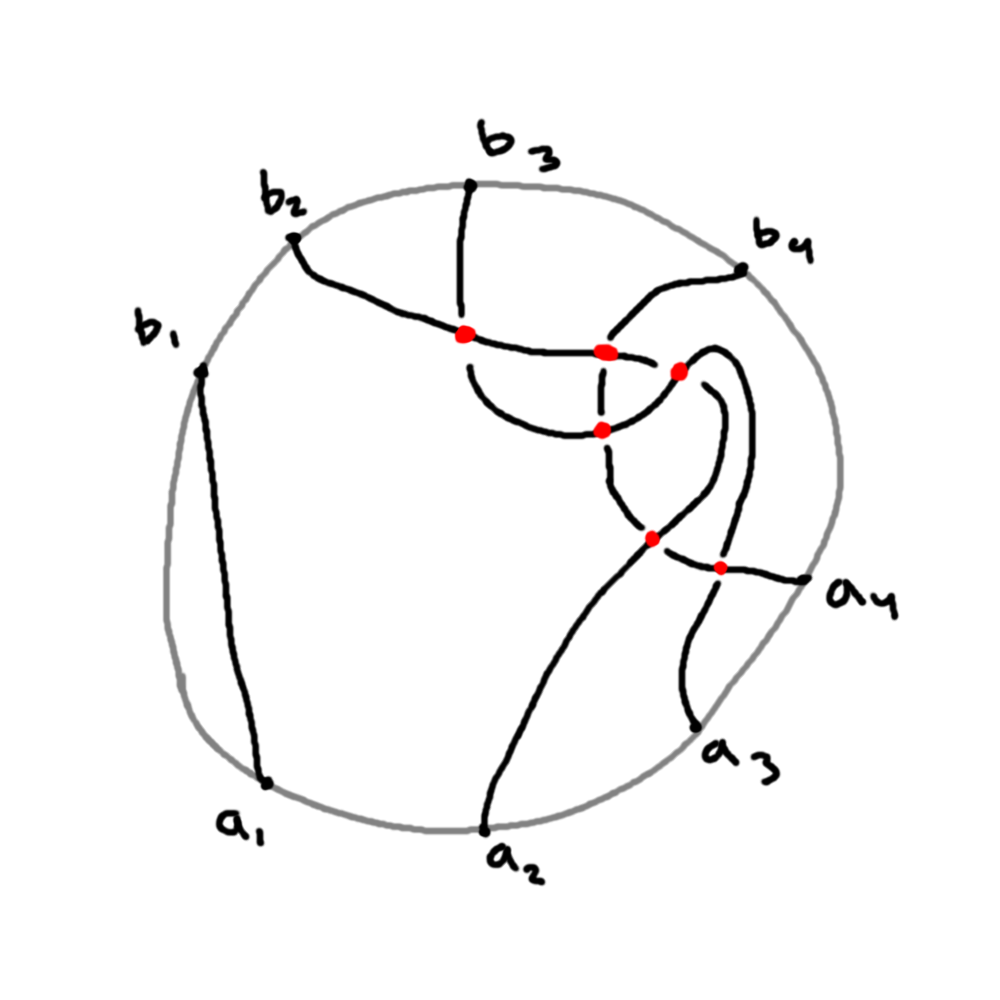
\includegraphics[width=0.4\textwidth]{tangle_diagram.png}
\caption{An example of a tangle diagram, notice there are 8 labeled points on the boundary (in grey) and each crossing (in red) is produced by at most two strands.}
\label{fig:tangle_diagram}
\end{figure}

The above definition is quite technical for the sake of clarity in how to generate a tangle diagram. In further discussions we will not use this level of precision, and simply focus on the combinatorial information of tangle diagrams, i.e. the relative position and orientation of the crossings. With regard to this combinatorial aspect there are maps or ``moves" that relate equivalent diagrams, those being the Reidermeister moves.


\subsection{Reidermeister moves, Tangles, the Tame and Wild}

\begin{definition}\textbf{(Reidermeister moves/ Isotopies)}
A region of a tangle diagram containing a configuration of strands and crossings as indicated in \Cref{fig:Rmoves} may be replaced by the associated configuration to produce a new tangle diagram. The new tangle diagram is equivalent to the old by a Reidermeister move.
\begin{figure}[h!]
\centering
\begin{subfigure}{0.31\textwidth}
\centering
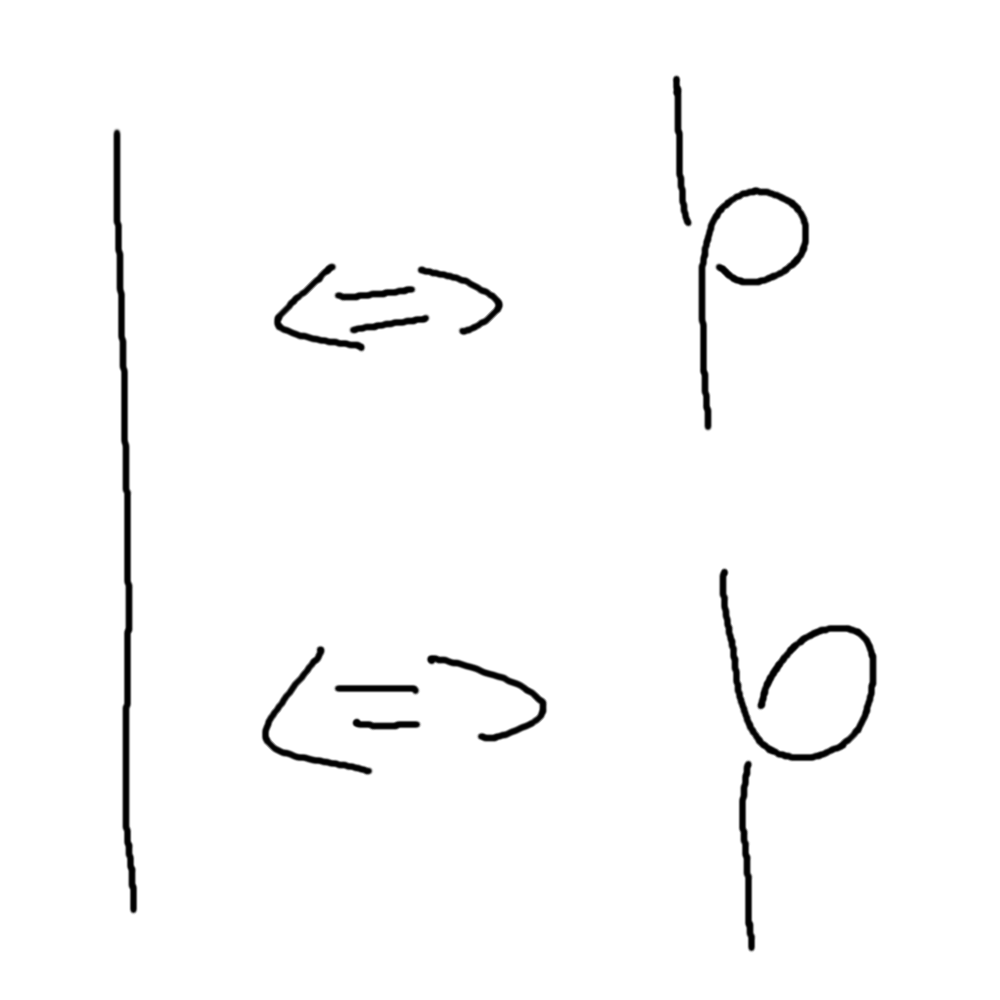
\includegraphics[width=\textwidth]{R1move.png}
\caption{The first move}
\label{fig:R1move}
\end{subfigure}
\hfill
\begin{subfigure}{0.31\textwidth}
\centering
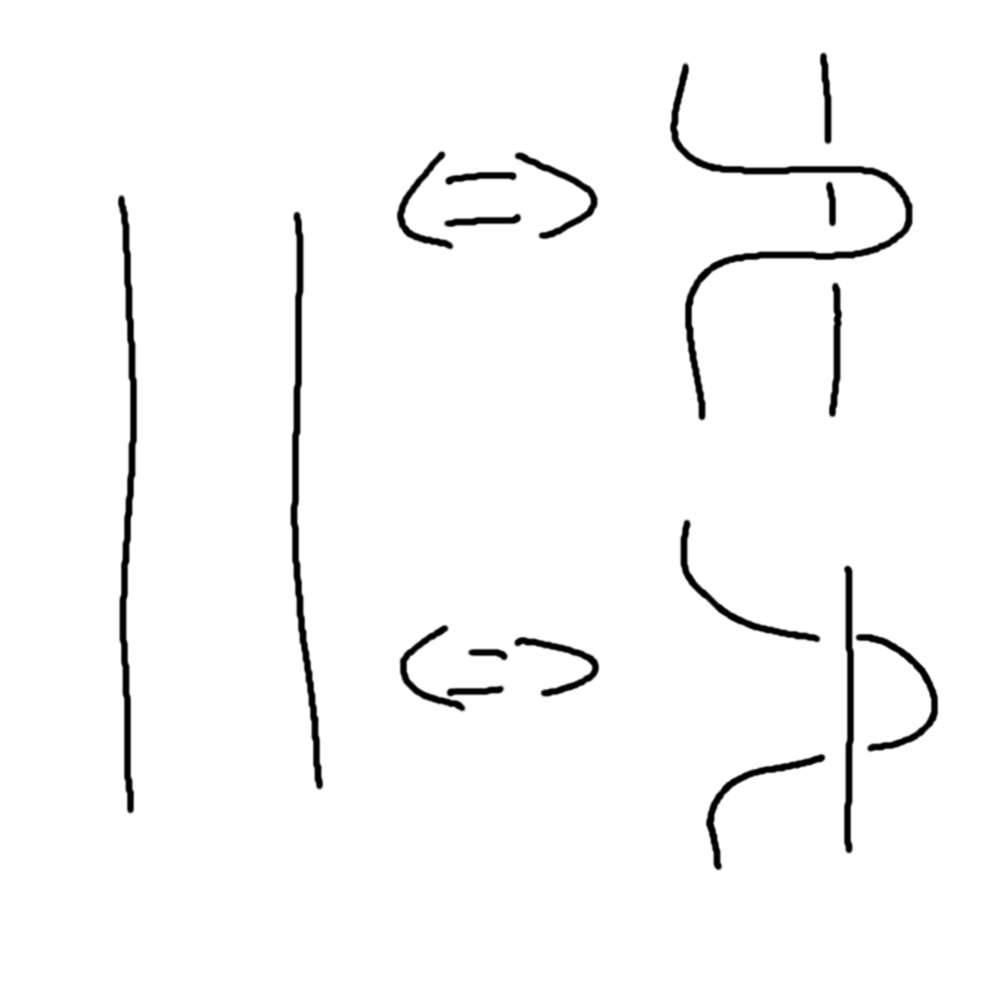
\includegraphics[width=\textwidth]{R2move.png}
\caption{The second move}
\label{fig:R2move}
\end{subfigure}
\hfill
\begin{subfigure}{0.31\textwidth}
\centering
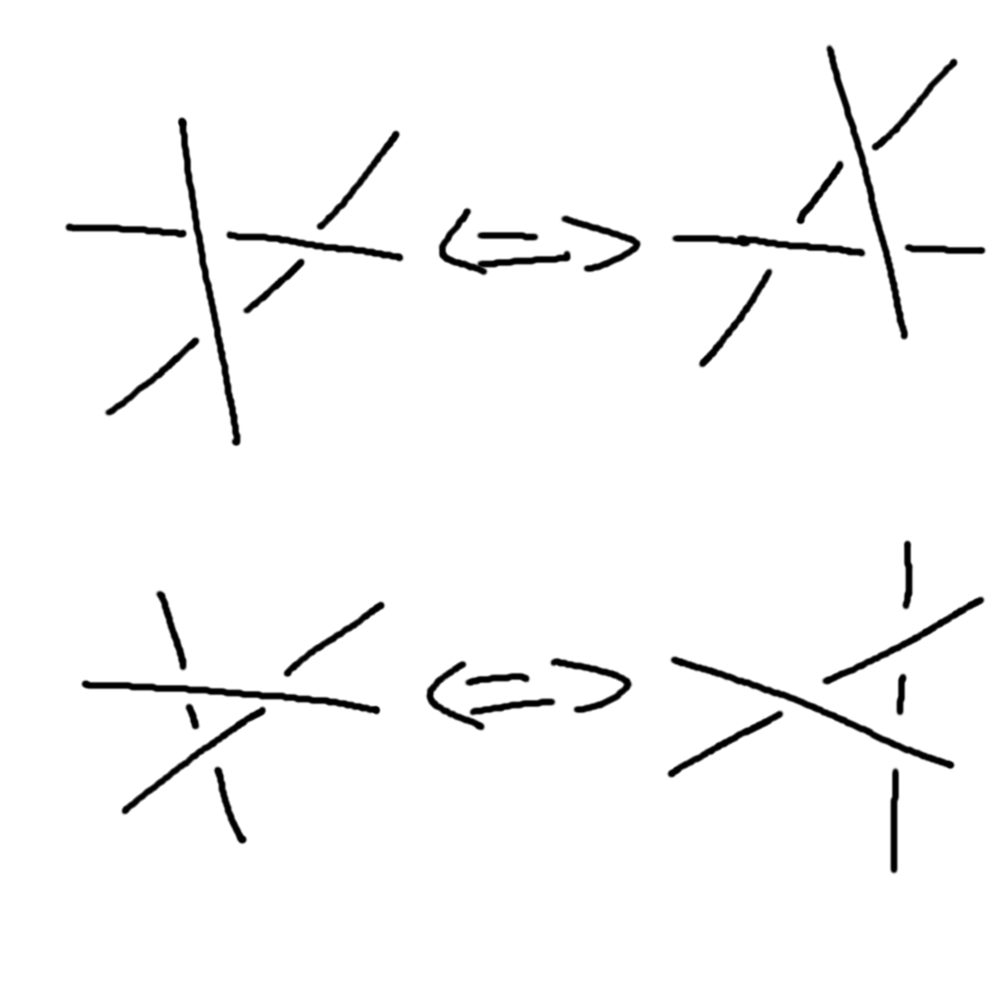
\includegraphics[width=\textwidth]{R3move.png}
\caption{The third move}
\label{fig:R3move}
\end{subfigure}
\caption{The 3 basic Reidermeister moves}
\label{fig:Rmoves}
\end{figure}
\end{definition}
The Reidermeister moves define an equivalence relation of tangle diagrams, which then defines an eqiuvalence class of tangle diagrams which we call a \textit{Tangle}. If we were to imagine tangle diagrams as tangible strands like shoelaces, and were to perform a sequence of Reidermeister moves, then intuitively we see that we either complicate or simplify the diagram but if were to take the ends of the laces and pull, ignoring friction, we get the same shape no matter what Reidermeister moves we apply.

\begin{definition}
A Tangle is an equivalence class of tangle diagrams under the relation of Reidermeister moves.
\end{definition}
Lastly we need to make a distinction between two varieties of tangle diagrams that our definition permits. Typically, when working with tangle diagrams we assume that the strands are either smooth or that they are homeomorphic to a finite polygonal chain, i.e. the strands are made from finitely many line segments, that way we can avoid pathological situations that are hard to understand, with this in mind we make this distinction a definition 

\begin{definition}
A tangle the strands of which are homeomorphic to a finite polygonal chain is called a \textit{Tame Tangle}. A tangle that is not tame is a \textit{Wild Tangle}.
\end{definition}

One might wonder why this condition was not included into the definition of a tangle diagram, and it will become clear once we discuss the algorithm in the next subsection. Before this we must mention orientations on diagrams and OU tangle diagrams.

\subsection{Oriented Gauss notation, OU diagrams}

As mentioned before we focus on the combinatorial information of a tangle diagram, so we ignore the parametrizations of each strand, and only care about the crossings and how they appear on the strands. We may abstract our diagrams to hold only this information, to do so we chose the Oriented Gauss notation or Oriented Gauss code. To produce the Oriented Gauss code we follow the steps:

\begin{enumerate}
\item Prescribe an order to the strands
\item For each strand prescribe an orientation, this is typically given by the map $\phi_i$ associated to the strand in question,
\item For each crossing assign a name, typically a unique integer, and a sign either $+$ or $-$ taking into account the orientations of the strands as shown in \Cref{fig:crossing},
\item For each strand associate a string of symbols by following from the start point to the end point and for each crossing we encounter we record either the symbol $O^s_i$ or $U^s_i$ where $O$ for over if our current strand is over, $U$ for under, $s$ for the sign of the crossing, and $i$ the name of the crossing encountered.
\item The ordered set of the previously recorded strings is called the Oriented Gauss code.
\end{enumerate}

\begin{figure}[h!]
\centering
\begin{subfigure}{0.20\textwidth}
\centering
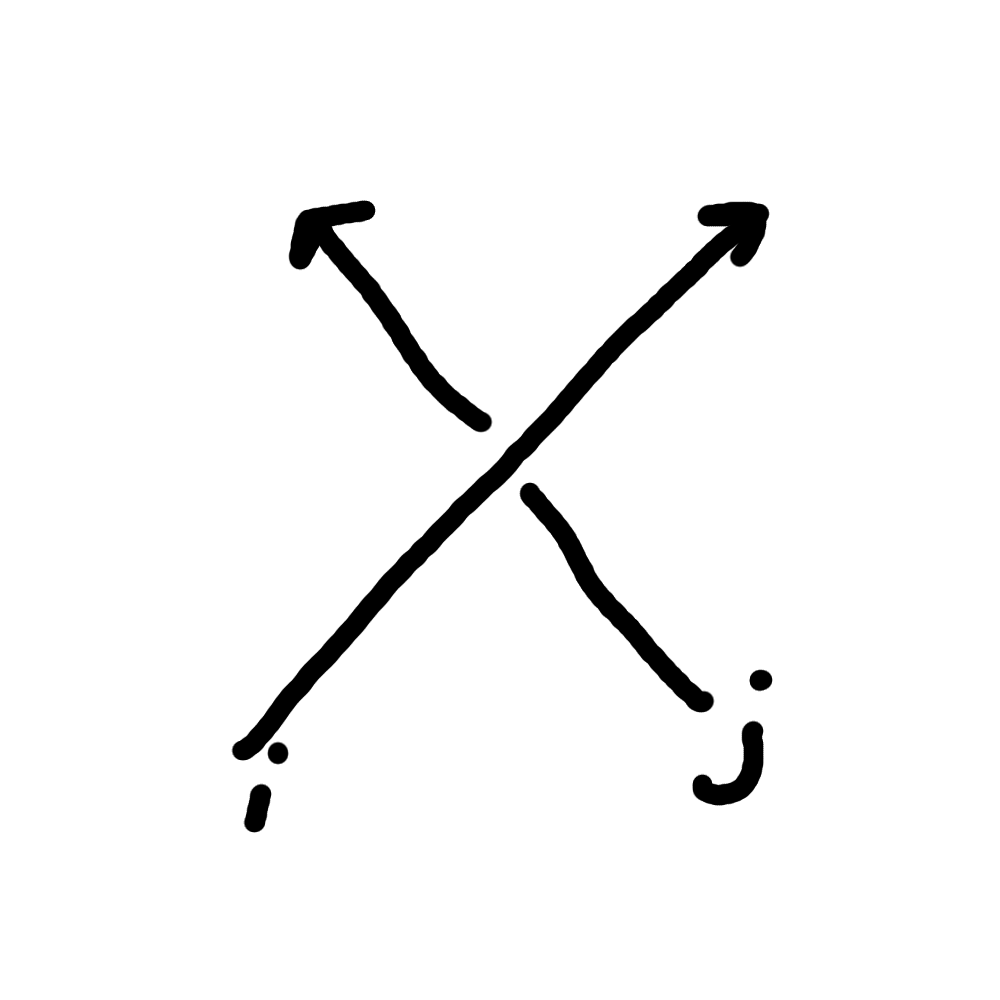
\includegraphics[width=\textwidth]{crossing+1.png}
\caption{This crossing is assigned +}
\label{fig:crossing:+1}
\end{subfigure}
\hspace{1cm}
\begin{subfigure}{0.20\textwidth}
\centering
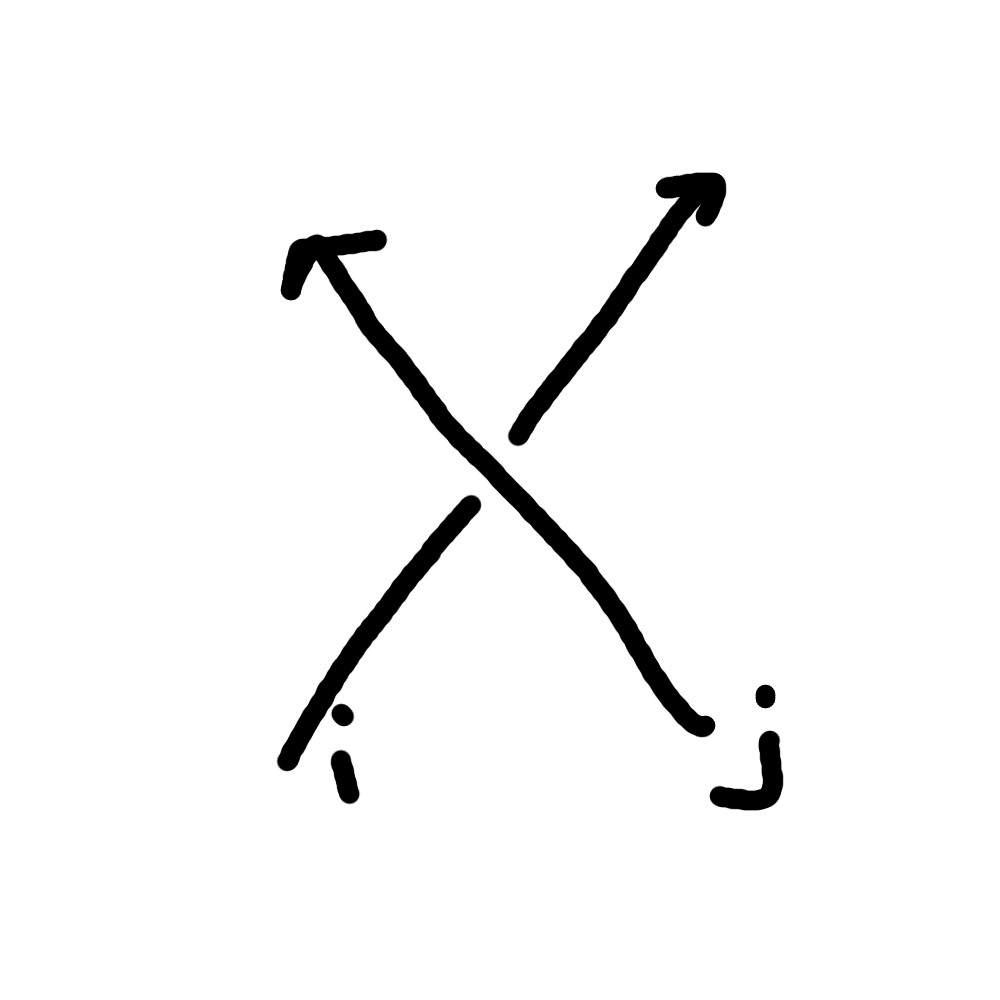
\includegraphics[width=\textwidth]{crossing-1.png}
\caption{This crossing is assigned -}
\label{fig:crossing:-1}
\end{subfigure}
\caption{Types of crossings by orientation.}
\label{fig:crossing}
\end{figure}

We provide some examples of tangles and their Oriented Gauss codes in \Cref{fig:Gaussexamples}

\begin{figure}[h!]
\centering
\begin{subfigure}{0.31\textwidth}
\centering
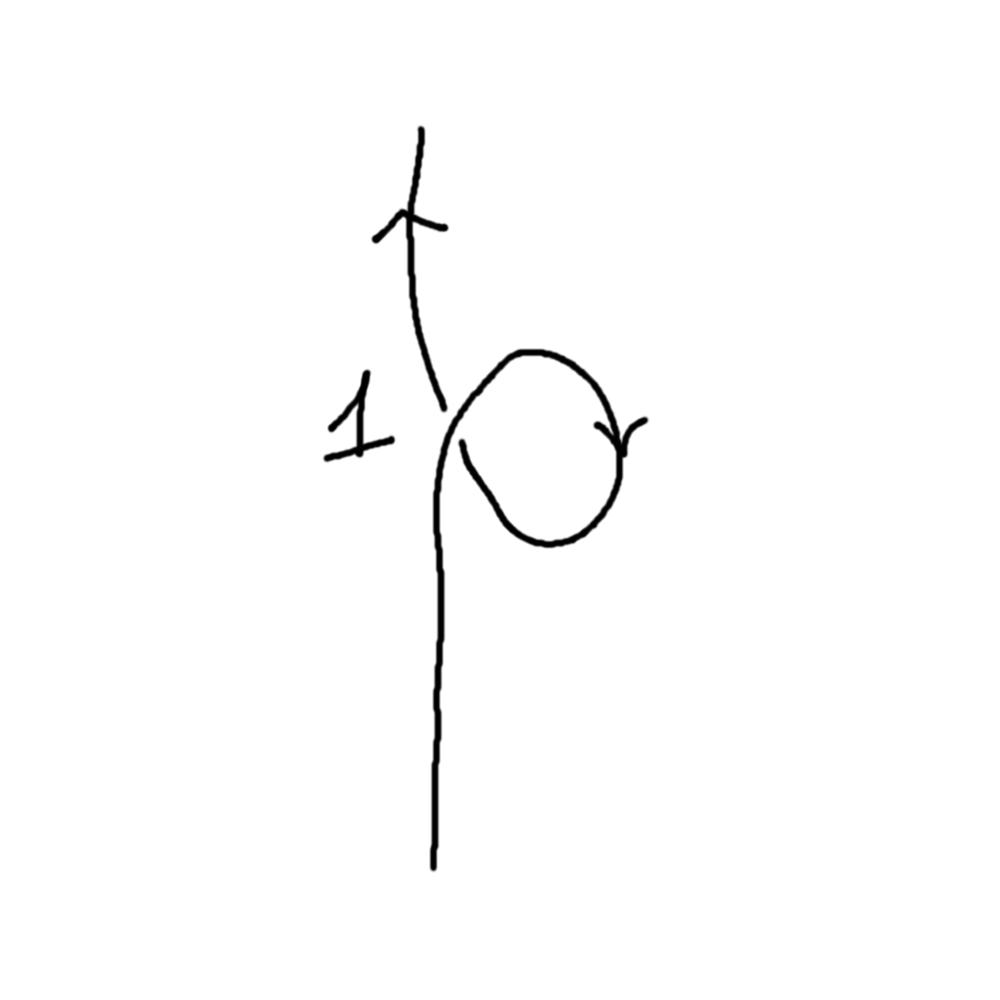
\includegraphics[width=\textwidth]{loop.png}
\caption{$O^{+}_1U^{+}_1$}
\label{fig:loop}
\end{subfigure}
\hfill
\begin{subfigure}{0.31\textwidth}
\centering
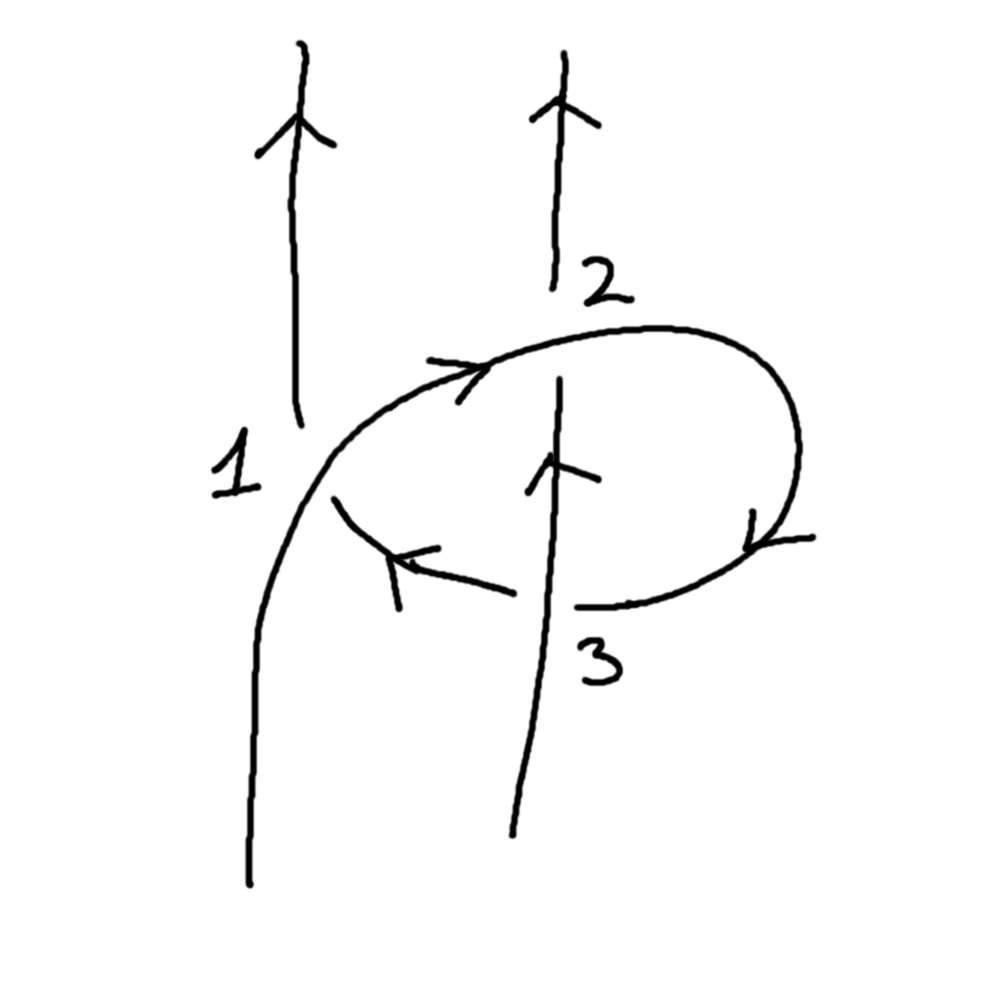
\includegraphics[width=\textwidth]{exampletangle.png}
\caption{$O_1^+O_2^+U_3^+U_1^+,O_3^+U_2^+$ where the left strand is first}
\label{fig:exampletangle}
\end{subfigure}
\hfill
\begin{subfigure}{0.31\textwidth}
\centering
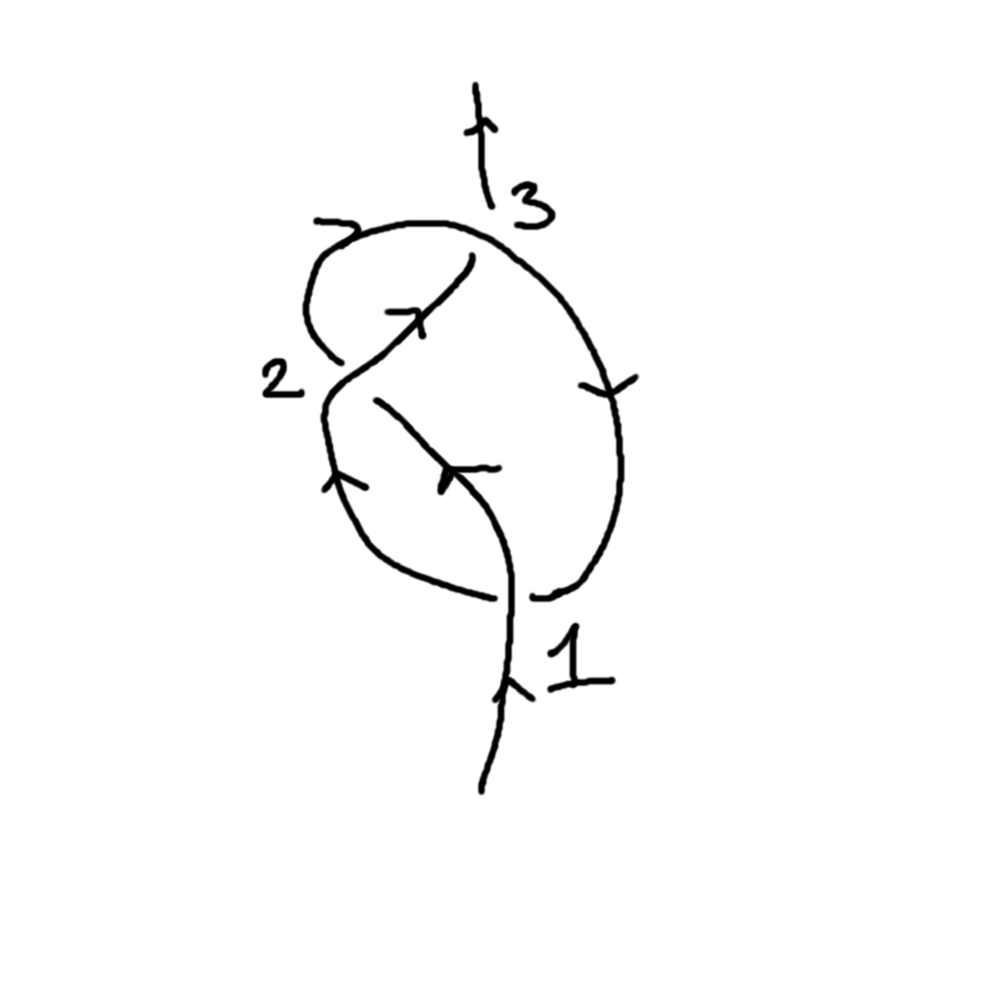
\includegraphics[width=\textwidth]{trefexample.png}
\caption{$O_1^+U_2^+O_3^+U_1^+O_2^+U_3^+$}
\label{fig:trefexample}
\end{subfigure}
\caption{Some examples of Oriented Gauss codes}
\label{fig:Gaussexamples}
\end{figure}

With the Oriented Gauss code we can now define an OU tangle diagram.

\begin{definition}
An OU tangle diagram is a tangle diagram with an Oriented Gauss code, the strings of which can be split in two substrings where the first consists of all $O$s and the second consists of $U$s
\end{definition}

We find an example of an OU tangle diagram in \Cref{fig:exampletangle}, the first string can be split into the substrings $O_1^+O_2^+$ and $U_3^+U_1^+$, the second string can be split into substrings $O_3^+$ and $U_2^+$, hence the diagram is indeed OU. Likewise \Cref{fig:loop} is also an OU tangle diagram, however \Cref{fig:trefexample} is not, since the $O$s and $U$s are mixed together.
